% Fibonacci-Pell nearest gaps: an all-exponent classification and
% quadratic-unit orbit rigidity
%
% Authors:
%   Dr. Denys Dutykh (Mathematics Department, Khalifa University of Science
%   and Technology, Abu Dhabi, UAE)
%   Prof. Laurent Vuillon (Univ. Savoie Mont Blanc, CNRS, LAMA, Chambery,
%   France)
%
\section{Quadratic units and the intrinsic nearest-gap system}
\label{sec:system}

This section builds the arithmetic dictionary used throughout the paper. A
candidate window is an Archimedean inequality; a target is a candidate whose
two coefficient coordinates also satisfy the exact norm--content equation.
Keeping those two levels separate is essential.

\subsection{Quadratic integers and primitive-unit normalisation}

We use the Fibonacci sequence

\begin{equation}
 F_0=0,
 \qquad
 F_1=1,
 \qquad
 F_{r+2}=F_{r+1}+F_r,
 \label{eq:fibonacci}
\end{equation}

and the Pell coordinates defined for every $r\in\Z$ by

\begin{equation}
 \lambda^r=C_r+P_r\sqrt2,
 \qquad
 \lambda=1+\sqrt2.
 \label{eq:pell-coordinates}
\end{equation}

Thus $P_0=0$, $P_1=1$, $P_{r+2}=2P_{r+1}+P_r$, and
$C_r=P_r+P_{r-1}$ for $r\geqslant1$. Since
$\overline\lambda=1-\sqrt2=-\lambda^{-1}$,

\begin{equation}
 C_r^2-2P_r^2=(-1)^r.
 \label{eq:pell-norm}
\end{equation}

Multiplication by $\lambda^r$ acts on coefficient columns by the integral
matrix

\begin{equation}
 \begin{pmatrix}C_r&2P_r\\ P_r&C_r\end{pmatrix},
 \label{eq:unit-matrix}
\end{equation}

whose determinant is $(-1)^r$. It therefore preserves coefficient content.
Equivalently, for $\alpha\in\Z[\sqrt2]$, $\cont\alpha$ is the largest
positive integer $c$ such that $\alpha\in c\Z[\sqrt2]$, and multiplication
by a unit is a unimodular change of the coefficient lattice.

There is also a useful arithmetic-geometric reading. The Pell conic
$X^2-2Y^2=1$ is the norm-one torus for $\Q(\sqrt2)/\Q$, while
$X^2-2Y^2=-1$ is its norm-$-1$ torsor. The coefficient-primitive integral
points on the latter with positive principal embedding are precisely
$\lambda^j$ for odd $j\in\Z$.
Thus the target condition below says that the primitive direction of a gap
lands on this torsor; see, for example, the Pell-conic viewpoint in
\cite[Chapter~7]{Lemmermeyer2021}.

More explicitly, the regular representation

\begin{equation}
 \iota(a+b\sqrt2)=
 \begin{pmatrix}a&2b\\ b&a\end{pmatrix},
 \qquad
 \det\iota(a+b\sqrt2)=a^2-2b^2,
 \label{eq:regular-representation}
\end{equation}

identifies the integral points of the norm-one torus with the rank-one
arithmetic group

\begin{equation}
 T(\Z)=\{\pm\lambda^{2m}:m\in\Z\}.
 \label{eq:norm-one-arithmetic-group}
\end{equation}

The norm-$-1$ integral fibre is the coset $\lambda T(\Z)$. Hence a target
gap is a rational lattice multiple of a point in this coset, and division by
the coefficient content recovers its primitive arithmetic-group direction.
This also explains why the matrix in \cref{eq:unit-matrix} preserves content:
it is the integral regular representation of a unit.

For the rest of the paper let

\begin{equation}
 f=F_q,
 \qquad
 x=F_{q+1},
 \qquad
 k=R_q=2x^2-f^2,
 \label{eq:f-x-k}
\end{equation}

and define

\begin{equation}
 A_q=f+x\sqrt2,
 \qquad
 B_q=x\sqrt2-f.
 \label{eq:A-B}
\end{equation}

For $q\geqslant1$, both numbers are positive and $A_qB_q=k$. The two signs
in \cref{eq:intro-D} are simply $D_{q,1}=A_q$ and
$D_{q,-1}=B_q$.

\begin{lemma}[Uniqueness and unit normalisation]
\label{lem:normalisation}
For a fixed pair $(q,\sigma)$ with $q\geqslant1$, at most one positive
integer $n$ satisfies

\begin{equation}
 D_{q,\sigma}^2<\lambda^n<2D_{q,\sigma}^2.
 \label{eq:nearest-window}
\end{equation}

If this integer exists, put $\Delta=\lambda^n-D_{q,\sigma}^2$ and
$g=\cont\Delta$. Then

\begin{equation}
 \norm\Delta=-g^2
 \label{eq:norm-content}
\end{equation}

if and only if

\begin{equation}
 \Delta=g\lambda^j
 \label{eq:normalised-unit}
\end{equation}

for a unique odd integer $j$. In that case $M=n-j$ is positive and
$M\equiv n-1\pmod2$.
\end{lemma}

\begin{proof}
The ratio of two distinct integral powers of $\lambda$ is at least
$\lambda>2$, proving uniqueness. If \cref{eq:norm-content} holds, then
$\Delta/g$ is a coefficient-primitive algebraic integer of norm $-1$ and
positive principal embedding. The unit group of $\Z[\sqrt2]$ gives
$\Delta/g=\lambda^j$ for one odd $j$. The converse is immediate from
\cref{eq:pell-norm}. Finally,
$\lambda^j=\Delta/g<\lambda^n$, so $j<n$ and $M=n-j>0$; the congruence for
$M$ follows because $j$ is odd.
\end{proof}

\begin{proposition}[Global parity selector]
\label{prop:parity-selector}
Every target satisfies

\begin{equation}
 n\text{ odd}\Longrightarrow3\mid q,
 \qquad
 n\text{ even}\Longrightarrow3\nmid q.
 \label{eq:parity-selector}
\end{equation}
\end{proposition}

\begin{proof}
The coefficient pair of the gap is

\begin{equation}
 \bigl(C_n-(f^2+2x^2),\ P_n-2\sigma fx\bigr).
 \label{eq:gap-coefficients}
\end{equation}

Modulo $2$, one has $C_n\equiv1$, $P_n\equiv n$, and
$f^2+2x^2\equiv f$. If the target condition holds, the quotient by the
content is an odd power of $\lambda$, whose two coefficients are odd.
Consequently the two entries in \cref{eq:gap-coefficients} have the same
parity, and

\begin{equation}
 n\equiv1-F_q\pmod2.
\end{equation}

The Fibonacci number $F_q$ is even exactly when $3\mid q$, proving
\cref{eq:parity-selector}.
\end{proof}

The selector is a conclusion, not an external admissibility hypothesis. The
even branch automatically has $3\nmid q$, hence $f$ and $k$ are odd and
$M$ is odd. Those are precisely the hypotheses used by the primitive
reconstruction below. The odd branch has a different factorisation and will
be treated in \cref{sec:odd-exponents}.

\subsection{Candidate windows are abundant}

Before imposing the norm--content equation, it is useful to know how often
the Archimedean window itself occurs. This separates the elementary supply
of candidates from the arithmetic rigidity that eventually leaves only two
targets. Put

\begin{equation}
 \vartheta=\log_\lambda\sqrt2,
 \qquad
 \eta=\log_\lambda\left(
  \frac{\sqrt2\varphi+1}{\lambda(\sqrt2\varphi-1)}
 \right),
 \qquad
 \varphi=\frac{1+\sqrt5}{2}.
 \label{eq:window-phases}
\end{equation}

\begin{theorem}[Exact density of the even candidate windows]
\label{thm:candidate-density}
Call the sign $\sigma$ available at $q$ if an even positive integer $n$
satisfies \cref{eq:nearest-window}. Then

\begin{equation}
 0<\eta<\vartheta<\frac12,
 \label{eq:phase-order}
\end{equation}

and the four sign patterns have natural densities

\begin{equation}
\begin{array}{lcccc}
 \toprule
 \text{available signs}&\text{both}&\text{plus only}&\text{minus only}&\text{neither}\\
 \midrule
 \text{density}&\vartheta-\eta&\eta&\eta&1-\vartheta-\eta\\
 \bottomrule
\end{array}
\label{eq:window-densities}
\end{equation}

The same relative densities hold after restricting $q$ to any fixed
arithmetic progression. In particular, they remain valid on either class
$q\equiv1,2\pmod3$ and on their union $3\nmid q$.
\end{theorem}

\begin{proof}
Write $x_\sigma(q)=\log_\lambda D_{q,\sigma}$. If $n=2m$, then
\cref{eq:nearest-window} is equivalent, away from its strict endpoints, to

\begin{equation}
 \{x_\sigma(q)\}\in I,
 \qquad
 I=(1-\vartheta,1).
 \label{eq:single-window-interval}
\end{equation}

Binet's formula gives

\begin{equation}
 x_\sigma(q)=q\gamma+\beta_\sigma+O(\varphi^{-2q}),
 \qquad
 \gamma=\frac{\log\varphi}{\log\lambda},
 \qquad
 \beta_\sigma=\log_\lambda\left(
  \frac{\sqrt2\varphi+\sigma}{\sqrt5}
 \right).
 \label{eq:window-binet-phase}
\end{equation}

The number $\gamma$ is irrational. Indeed, a rational relation would put
equal positive powers of $\varphi$ and $\lambda$ in
$\Q(\sqrt5)\cap\Q(\sqrt2)=\Q$, whereas no positive power of $\varphi$ is
rational. Hence $q\gamma+\beta_-$ is equidistributed modulo one by Weyl's
theorem \cite{Weyl1916}. Equivalently, its empirical measures converge to
Haar probability measure on $\R/\Z$. Since

\begin{equation}
 \beta_+-\beta_-=1+\eta,
\end{equation}

the minus interval is $I_-=(1-\vartheta,1)$ and the plus interval, expressed
in the same phase coordinate, is

\begin{equation}
 I_+=(1-\vartheta-\eta,1-\eta).
 \label{eq:two-window-intervals}
\end{equation}

The endpoint order in \cref{fig:phase-partition} gives the four lengths in
\cref{eq:window-densities}; these lengths are exactly the Haar measures of
the corresponding phase regions. The inequalities in
\cref{eq:phase-order} reduce respectively to
$1+\sqrt2>\sqrt5$, $\varphi>3/2$, and $\lambda>2$. The exponentially
decaying error in \cref{eq:window-binet-phase} can change membership only
near the four endpoints, a set of density zero. On a progression
$q=q_0+Q\ell$, the increment $Q\gamma$ remains irrational, so the same
argument applies.
\end{proof}

There is an exact probability interpretation of this deterministic theorem.
If $Q_N$ is chosen uniformly from $\{1,\ldots,N\}$, then the four
availability events converge to the probabilities in
\cref{eq:window-densities}. The probability space is simply the phase circle
with Haar measure; no independence assumption or random mechanism enters
the arithmetic.

\begin{figure}[H]
\centering
\begin{tikzpicture}[x=0.97cm,y=1cm,>=Stealth]
 \draw[very thick] (0,0)--(12.8,0);
 \foreach \x in {0,6.96,7.77,11.99,12.8}
   \draw[very thick] (\x,-0.08)--(\x,0.08);
 \fill[black!6] (0,0.12) rectangle (6.96,0.42);
 \fill[black!18] (6.96,0.12) rectangle (7.77,0.42);
 \fill[black!35] (7.77,0.12) rectangle (11.99,0.42);
 \fill[black!18] (11.99,0.12) rectangle (12.8,0.42);
 \node[below] at (0,-0.08) {$0$};
 \node[below left] at (6.96,-0.08) {$1-\vartheta-\eta$};
 \node[below right] at (7.77,-0.50) {$1-\vartheta$};
 \draw[thin] (7.77,-0.08)--(7.77,-0.48);
 \node[below] at (11.99,-0.08) {$1-\eta$};
 \node[below] at (12.8,-0.08) {$1$};
 \node at (3.48,0.27) {neither};
 \node at (9.88,0.27) {both};
 \node[above left] (po) at (6.65,0.72) {plus only};
 \draw[-Stealth,thin] (po.east)--(7.36,0.43);
 \node[above] (mo) at (13.15,1.80) {minus only};
 \draw[-Stealth,thin] (mo.south)--(12.72,0.45);
 \draw[blue!65!black,very thick] (6.96,1.55)--(11.99,1.55);
 \draw[blue!65!black] (6.96,1.42)--(6.96,1.68)
   (11.99,1.42)--(11.99,1.68);
 \node[blue!65!black,above] at (9.48,1.55) {$I_+$};
 \draw[black,very thick] (7.77,1.08)--(12.8,1.08);
 \draw[black] (7.77,0.95)--(7.77,1.21)
   (12.8,0.95)--(12.8,1.21);
 \node[above] at (10.29,1.08) {$I_-$};
\end{tikzpicture}
\caption{The exact phase partition for the two even nearest-window
candidates. Irrational rotation distributes the limiting phase uniformly;
the four natural densities are therefore the displayed interval lengths.
Availability is only an Archimedean condition and does not imply the exact
norm--content equation.}
\label{fig:phase-partition}
\end{figure}

Numerically, $\vartheta=0.3932198506\ldots$ and
$\eta=0.0631959999\ldots$, so both windows occur for about $33\%$ of all
indices. The final classification will show that this positive-density
supply contains only two norm--content targets. Scarcity of candidate
windows is therefore not the exclusion mechanism.

\subsection{Primitive reconstruction in the even branch}

The next reconstruction is the geometric input behind the later height
separation. We include the proof because using an arbitrary divisor of
$(k^2-1)/4$ here would be invalid.

\begin{lemma}[Primitive rectangle reconstructed from a target]
\label{lem:rectangle}
Assume that $n$ is even and that
\cref{eq:nearest-window,eq:norm-content} hold. With $M=n-j$,
there is an odd integer $W$ such that

\begin{equation}
 W^2=C_M^2+1-k^2,
 \qquad
 \gcd(k,W)=1,
 \qquad
 \abs W<C_M.
 \label{eq:W-relation}
\end{equation}

Put

\begin{equation}
 U=\frac{C_M-W}{2},
 \qquad
 V=\frac{C_M+W}{2}.
 \label{eq:UV}
\end{equation}

Then $U,V$ are positive integers of opposite parity and

\begin{equation}
 UV=\frac{k^2-1}{4}.
 \label{eq:UV-product}
\end{equation}

Moreover, $g/2$ equals $U$ on the plus branch and $V$ on the minus branch,
and

\begin{equation}
 g<k,
 \qquad
 U\geqslant\sqrt{k},
 \qquad
 V\geqslant\sqrt{k}.
 \label{eq:factor-lower}
\end{equation}
\end{lemma}

\begin{proof}
On the plus branch, division of
$\lambda^n-A_q^2=g\lambda^j$ by $\lambda^j$ gives

\begin{equation}
 A_q^2\lambda^{-j}=C_M-g+P_M\sqrt2.
 \label{eq:plus-orbit}
\end{equation}

On the minus branch the same calculation gives

\begin{equation}
 B_q^2\lambda^{-j}=C_M-g+P_M\sqrt2.
 \label{eq:minus-orbit}
\end{equation}

Define $W=C_M-g$ in \cref{eq:plus-orbit} and $W=g-C_M$ in
\cref{eq:minus-orbit}; thus the rational coefficient in those two equations
is, respectively, $W$ and $-W$. The upper half of the strict window gives
$D_{q,\sigma}^2>\lambda^n/2$, and therefore

\[
 g\lambda^j=\lambda^n-D_{q,\sigma}^2<\frac{\lambda^n}{2}.
\]

Thus $2g<\lambda^{n-j}=\lambda^M$. Since $M$ is odd,

\begin{equation}
 \frac{\lambda^M}{2}=C_M+\frac{\lambda^{-M}}2<C_M+1.
\end{equation}

Thus $g\leqslant C_M$. Equality would give $W=0$ and
$k^2=C_M^2+1$, which is impossible modulo $8$ because $k$ and $C_M$ are
odd. Therefore \cref{eq:W-relation} has $\abs W=C_M-g<C_M$.

Taking norms in \cref{eq:plus-orbit,eq:minus-orbit} and using
\cref{eq:pell-norm} proves the first equality in \cref{eq:W-relation}. To
prove primitivity, suppose that an odd prime $p$ divides both $k$ and $W$.
The norm relation then gives $p\mid P_M$. After multiplication by a Pell
unit, $p$ would divide both coefficients of $A_q^2$ or $B_q^2$. Those
coefficients are $f^2+2x^2$ and $2fx$ up to signs. Since
$\gcd(f,x)=1$ and $p\mid2x^2-f^2$, this is impossible. Hence
$\gcd(k,W)=1$.

Factoring $C_M^2-W^2=k^2-1$ proves
\cref{eq:UV-product}. Since $M$ and $k$ are odd, the norm relation shows
that $W$ is odd. Hence $U+V=C_M$ is odd, so $U$ and $V$ have opposite
parities. Put

\begin{equation}
 X_\delta=\frac{k-\delta}{2},
 \qquad
 Y_\delta=\frac{k+\delta}{2}.
\end{equation}

The two factors $X_\delta$ and $Y_\delta$ are coprime and consecutive.
Choose the unique $\delta\in\{1,-1\}$ for which $Y_\delta$ is even when
$U$ is even, and $X_\delta$ is even when $V$ is even. Define

\begin{equation}
 a=\gcd(U,X_\delta),
 \qquad
 d=\gcd(U,Y_\delta),
 \qquad
 S=\frac{X_\delta}{a},
 \qquad
 T=\frac{Y_\delta}{d}.
 \label{eq:rectangle-construction}
\end{equation}

Because $X_\delta Y_\delta=UV$ and
$\gcd(X_\delta,Y_\delta)=1$, every prime power in $U$ occurs wholly in
exactly one of $X_\delta,Y_\delta$. Therefore
$\gcd(U,X_\delta)\gcd(U,Y_\delta)=U$, and
\cref{eq:rectangle-construction} gives

\begin{equation}
 U=ad,
 \qquad
 V=ST,
 \qquad
 aS=X_\delta,
 \qquad
 dT=Y_\delta,
 \qquad
 dT-aS=\delta.
\label{eq:rectangle}
\end{equation}

\Cref{fig:primitive-rectangle} shows the factor rectangle that
\cref{eq:rectangle} describes.

\begin{figure}[t]
\centering
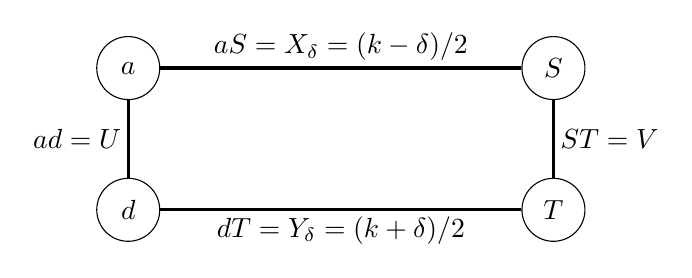
\begin{tikzpicture}[
 factor/.style={circle,draw,minimum size=8mm,inner sep=1pt},
 lab/.style={fill=white,inner sep=2pt}
]
 \node[factor] (a) at (0,1.8) {$a$};
 \node[factor] (S) at (5.4,1.8) {$S$};
 \node[factor] (d) at (0,0) {$d$};
 \node[factor] (T) at (5.4,0) {$T$};
 \draw[very thick] (a)--node[lab,above] {$aS=X_\delta=(k-\delta)/2$} (S);
 \draw[very thick] (d)--node[lab,below] {$dT=Y_\delta=(k+\delta)/2$} (T);
 \draw[very thick] (a)--node[lab,left] {$ad=U$} (d);
 \draw[very thick] (S)--node[lab,right] {$ST=V$} (T);
\end{tikzpicture}
\caption{The primitive factor rectangle. Coprimality of the consecutive
horizontal products allocates every prime power to one corner in each row.
The opposite-corner quadratic factors $S^2+d^2$ and
$(T^2+a^2)/2$ are coprime by \cref{eq:conic-coprime}, allowing Lagrange's
identity to force two conics.}
\label{fig:primitive-rectangle}
\end{figure}

The same prime-support separation gives

\begin{equation}
 \gcd(a,d)=\gcd(a,T)=\gcd(S,d)=\gcd(S,T)=1.
 \label{eq:rectangle-cross-coprime}
\end{equation}

Our choice of $\delta$ makes $a,T$ odd and makes $S,d$ of opposite parity.
We claim that

\begin{equation}
 \gcd\left(S^2+d^2,\frac{T^2+a^2}{2}\right)=1.
 \label{eq:conic-coprime}
\end{equation}

Both factors are odd. If an odd prime $p$ divided them, then none of
$a,d,S,T$ would vanish modulo $p$. Put
$r=S/d$ and $s=T/a$ in $\mathbb{F}_p$. The two norm congruences give
$r^2=s^2=-1$. The relation $dT-aS=\delta$ shows that $r\ne s$, so
$s=-r$. It follows that
$k=aS+dT=ad(r+s)$ and $W=ST-ad=ad(rs-1)$ both vanish modulo $p$, contrary
to $\gcd(k,W)=1$. This proves \cref{eq:conic-coprime}.

We therefore have

\begin{equation}
 S^2+d^2=H^2,
 \qquad
 T^2+a^2=2J^2
 \label{eq:two-conics}
\end{equation}

for coprime positive integers $H,J$. One direct way to see the square
conclusion is Lagrange's identity:

\begin{equation}
 (S^2+d^2)\frac{T^2+a^2}{2}
 =\frac{(ad+ST)^2+(dT-aS)^2}{2}
 =P_M^2.
\end{equation}

The two factors on the left are coprime by \cref{eq:conic-coprime}, so each
is a square.

For the positive Pythagorean pair $(S,d)$, integrality gives
$H-S\geqslant1$ and $H-d\geqslant1$. Consequently

\begin{equation}
 d^2=(H-S)(H+S)\geqslant2S+1,
 \qquad
 S^2=(H-d)(H+d)\geqslant2d+1,
\end{equation}

or equivalently

\begin{equation}
 2S\leqslant d^2-1,
 \qquad
 2d\leqslant S^2-1.
\end{equation}

Using $k=2aS+\delta=2dT-\delta$, the preceding inequalities, and
positivity gives

\begin{align}
 k
 &\leqslant a(d^2-1)+1
 \leqslant ad^2
 \leqslant(ad)^2=U^2,
 \label{eq:U-lower}\\
 k
 &\leqslant T(S^2-1)+1
 \leqslant TS^2
 \leqslant(ST)^2=V^2.
 \label{eq:V-lower}
\end{align}

These inequalities prove the two factor bounds in
\cref{eq:factor-lower}. Finally, the
definitions of $W$ show $g=C_M-W=2U$ on the plus branch and
$g=C_M+W=2V$ on the minus branch. In each case the selected factor is the
smaller of $U,V$, so
$g<2\sqrt{UV}=\sqrt{k^2-1}<k$.
\end{proof}

\begin{remark}
The rectangle is reconstructed from the full coefficient-content target,
not from a numerical near equality. This is why the lower bound
\cref{eq:factor-lower} is available. The proof of the classification would
fail if $g/2$ were replaced by an arbitrary divisor of
$(k^2-1)/4$.
\end{remark}

With the arithmetic dictionary and the primitive rectangle in hand, we now
enter the even branch. We first determine which primitive-unit exponents can
lead, and then separate those exponents quantitatively from the nearest Pell
exponent.
